\documentclass[
	12pt,				% tamanho da fonte
	%openright,			% capítulos começam em pág ímpar (insere página vazia caso preciso)
	%twoside,			% para impressão em recto e verso. Oposto a oneside
	openany,			%Para nao pular folhas quando um paragrafo novo começa. Oposto de Twoside e openright
	a4paper,			% tamanho do papel.
	chapter=TITLE,		% títulos de capítulos convertidos em letras maiúsculas
	section=TITLE,		% títulos de seções convertidos em letras maiúsculas
	%subsection=TITLE,	% títulos de subseções convertidos em letras maiúsculas
	%subsubsection=TITLE,% títulos de subsubseções convertidos em letras maiúsculas
	english,
	brazil				% o último idioma é o principal do documento
]{abntex2}
\usepackage[brazil]{babel}
\usepackage[utf8]{inputenc} %Pacote de linguas
\usepackage[normalem]{ulem}
\usepackage[T1]{fontenc}
\usepackage{lipsum}
\usepackage{cmap}
\usepackage{graphicx}
\usepackage[brazilian,hyperpageref]{backref}
\usepackage[alf]{abntex2cite} % Citações padrão ABNT
\usepackage{rotating}
\usepackage{float}
\usepackage{color}
\usepackage{listings}    
\usepackage{inconsolata}

\usepackage{listings}

\newcommand{\imagem}[3]{
	\begin{figure}[htb]
		\begin{center}
			\includegraphics[scale=0.5]{#1}
		\end{center}
		\caption{#2}	%\label{#3}
	\end{figure}
}

\title{Sistemas operacionais II \\ Lista de exercícios 4}
\date{\today}
\autor{Felipe Menino Carlos}

\setlength{\parindent}{1.3cm}
\frenchspacing

% Adicionando idioma
\selectlanguage{brazil}

\begin{document}
\maketitle

\chapter{Exercícios}

\subsection{Exercício 1}

No diretório do seu usuário.
Para resolver o exercício o comando utilizado foi:

\begin{itemize}
\item cd 
\end{itemize}

\subsection{Exercício 2}

Crie 3 arquivos de texto. Os comandos executados foram os seguintes:

\begin{itemize}
	\item > arquivo1.sh 
	\item > arquivo2.sh
	\item > arquivo3.sh
\end{itemize}

\subsection{Exercício 3}

Escreva o conteúdo para cada arquivo, usando o vi.

\begin{itemize}
	\item{Arquivo 1}
		\begin{figure}[htp]
  			\centering
  			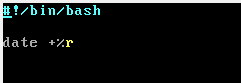
\includegraphics[scale=0.7]{exe3-1.png}
		\end{figure}
	\item{Arquivo 2}
		\begin{figure}[htp]
  			\centering
  			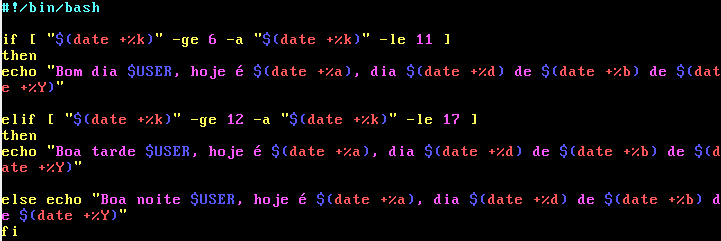
\includegraphics[scale=0.5]{exe3-2.png}
		\end{figure}
	\item{Arquivo 3}
		\begin{figure}[htp]
  			\centering
  			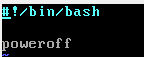
\includegraphics[scale=0.7]{exe3-3.png}
		\end{figure}
\end{itemize}

\subsection{Exercícios 4 e 5}

Os exercícios resolvidos são os seguintes:
\begin{itemize}
	\item Salve os arquivos com a extensão .sh. Por exemplo arquivo1.sh.
	\item Modifique a permissão dos arquivos para que eles possam ser executados apenas pelo dono e seu grupo.
\end{itemize}

Os comandos utilizados foram os seguintes:

\begin{itemize}
	\item chmod u=rwx,g=x,o=-rwx arquivo1.sh
	\item chmod u=rwx,g=x,o=-rwx arquivo2.sh
	\item chmod u=rwx,g=x,o=-rwx arquivo3.sh
\end{itemize}

\begin{figure}[htp]
  \centering
  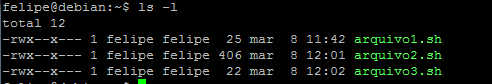
\includegraphics[scale=1]{exe5.png}
\end{figure}


\subsection{Exercício 6}

Para cada  arquivo  criado  execute  seu  conteúdo  usando  o  comando  ./arquivo.  Por exemplo: ./arquivo1.sh

\begin{figure}[htp]
  \centering
  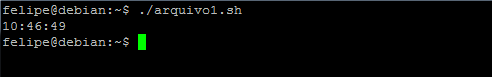
\includegraphics[scale=1]{exe6-1.png}
\end{figure}

\begin{figure}[htp]
  \centering
  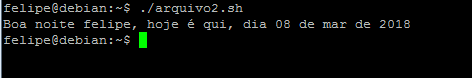
\includegraphics[scale=1]{exe6-2.png}
\end{figure}

\subsection{Exercício 7}

O terceiro arquivo deverá ser executado pelo usuário root.

Para resolver este exercício os seguintes comandos foram executados

\begin{itemize}
	\item su
	\item ./arquivo3.sh
\end{itemize}

\end{document}
